
%% bare_jrnl_compsoc.tex
%% V1.3
%% 2007/01/11
%% by Michael Shell
%% See:
%% http://www.michaelshell.org/
%% for current contact information.
%%
%% This is a skeleton file demonstrating the use of IEEEtran.cls
%% (requires IEEEtran.cls version 1.7 or later) with an IEEE Computer
%% Society journal paper.
%%
%% Support sites:
%% http://www.michaelshell.org/tex/ieeetran/
%% http://www.ctan.org/tex-archive/macros/latex/contrib/IEEEtran/
%% and
%% http://www.ieee.org/

%%*************************************************************************
%% Legal Notice:
%% This code is offered as-is without any warranty either expressed or
%% implied; without even the implied warranty of MERCHANTABILITY or
%% FITNESS FOR A PARTICULAR PURPOSE! 
%% User assumes all risk.
%% In no event shall IEEE or any contributor to this code be liable for
%% any damages or losses, including, but not limited to, incidental,
%% consequential, or any other damages, resulting from the use or misuse
%% of any information contained here.
%%
%% All comments are the opinions of their respective authors and are not
%% necessarily endorsed by the IEEE.
%%
%% This work is distributed under the LaTeX Project Public License (LPPL)
%% ( http://www.latex-project.org/ ) version 1.3, and may be freely used,
%% distributed and modified. A copy of the LPPL, version 1.3, is included
%% in the base LaTeX documentation of all distributions of LaTeX released
%% 2003/12/01 or later.
%% Retain all contribution notices and credits.
%% ** Modified files should be clearly indicated as such, including  **
%% ** renaming them and changing author support contact information. **
%%
%% File list of work: IEEEtran.cls, IEEEtran_HOWTO.pdf, bare_adv.tex,
%%                    bare_conf.tex, bare_jrnl.tex, bare_jrnl_compsoc.tex
%%*************************************************************************

% *** Authors should verify (and, if needed, correct) their LaTeX system  ***
% *** with the testflow diagnostic prior to trusting their LaTeX platform ***
% *** with production work. IEEE's font choices can trigger bugs that do  ***
% *** not appear when using other class files.                            ***
% The testflow support page is at:
% http://www.michaelshell.org/tex/testflow/




% Note that the a4paper option is mainly intended so that authors in
% countries using A4 can easily print to A4 and see how their papers will
% look in print - the typesetting of the document will not typically be
% affected with changes in paper size (but the bottom and side margins will).
% Use the testflow package mentioned above to verify correct handling of
% both paper sizes by the user's LaTeX system.
%
% Also note that the "draftcls" or "draftclsnofoot", not "draft", option
% should be used if it is desired that the figures are to be displayed in
% draft mode.
%
% The Computer Society usually requires 12pt for submissions.
%
\documentclass[12pt,journal,compsoc]{IEEEtran}
%
% If IEEEtran.cls has not been installed into the LaTeX system files,
% manually specify the path to it like:
% \documentclass[12pt,journal,compsoc]{../sty/IEEEtran}





% Some very useful LaTeX packages include:
% (uncomment the ones you want to load)


% *** MISC UTILITY PACKAGES ***
%
%\usepackage{ifpdf}
% Heiko Oberdiek's ifpdf.sty is very useful if you need conditional
% compilation based on whether the output is pdf or dvi.
% usage:
% \ifpdf
%   % pdf code
% \else
%   % dvi code
% \fi
% The latest version of ifpdf.sty can be obtained from:
% http://www.ctan.org/tex-archive/macros/latex/contrib/oberdiek/
% Also, note that IEEEtran.cls V1.7 and later provides a builtin
% \ifCLASSINFOpdf conditional that works the same way.
% When switching from latex to pdflatex and vice-versa, the compiler may
% have to be run twice to clear warning/error messages.
% Code listings
\newcommand{\code}[1]{\texttt{#1}}





% *** CITATION PACKAGES ***
%
\ifCLASSOPTIONcompsoc
  % IEEE Computer Society needs nocompress option
  % requires cite.sty v4.0 or later (November 2003)
  % \usepackage[nocompress]{cite}
  \usepackage{cite}
\else
  % normal IEEE
  \usepackage{cite}
\fi
% cite.sty was written by Donald Arseneau
% V1.6 and later of IEEEtran pre-defines the format of the cite.sty package
% \cite{} output to follow that of IEEE. Loading the cite package will
% result in citation numbers being automatically sorted and properly
% "compressed/ranged". e.g., [1], [9], [2], [7], [5], [6] without using
% cite.sty will become [1], [2], [5]--[7], [9] using cite.sty. cite.sty's
% \cite will automatically add leading space, if needed. Use cite.sty's
% noadjust option (cite.sty V3.8 and later) if you want to turn this off.
% cite.sty is already installed on most LaTeX systems. Be sure and use
% version 4.0 (2003-05-27) and later if using hyperref.sty. cite.sty does
% not currently provide for hyperlinked citations.
% The latest version can be obtained at:
% http://www.ctan.org/tex-archive/macros/latex/contrib/cite/
% The documentation is contained in the cite.sty file itself.
%
% Note that some packages require special options to format as the Computer
% Society requires. In particular, Computer Society  papers do not use
% compressed citation ranges as is done in typical IEEE papers
% (e.g., [1]-[4]). Instead, they list every citation separately in order
% (e.g., [1], [2], [3], [4]). To get the latter we need to load the cite
% package with the nocompress option which is supported by cite.sty v4.0
% and later. Note also the use of a CLASSOPTION conditional provided by
% IEEEtran.cls V1.7 and later.





% *** GRAPHICS RELATED PACKAGES ***
%
\ifCLASSINFOpdf
  \usepackage[pdftex]{graphicx}
  % declare the path(s) where your graphic files are
  \graphicspath{{./img/}}
  % and their extensions so you won't have to specify these with
  % every instance of \includegraphics
  \DeclareGraphicsExtensions{.pdf,.jpeg,.png}
\else
  % or other class option (dvipsone, dvipdf, if not using dvips). graphicx
  % will default to the driver specified in the system graphics.cfg if no
  % driver is specified.
  \usepackage[dvips]{graphicx}
  % declare the path(s) where your graphic files are
  \graphicspath{{./img/}}
  % and their extensions so you won't have to specify these with
  % every instance of \includegraphics
  \DeclareGraphicsExtensions{.eps}
\fi
% graphicx was written by David Carlisle and Sebastian Rahtz. It is
% required if you want graphics, photos, etc. graphicx.sty is already
% installed on most LaTeX systems. The latest version and documentation can
% be obtained at: 
% http://www.ctan.org/tex-archive/macros/latex/required/graphics/
% Another good source of documentation is "Using Imported Graphics in
% LaTeX2e" by Keith Reckdahl which can be found as epslatex.ps or
% epslatex.pdf at: http://www.ctan.org/tex-archive/info/
%
% latex, and pdflatex in dvi mode, support graphics in encapsulated
% postscript (.eps) format. pdflatex in pdf mode supports graphics
% in .pdf, .jpeg, .png and .mps (metapost) formats. Users should ensure
% that all non-photo figures use a vector format (.eps, .pdf, .mps) and
% not a bitmapped formats (.jpeg, .png). IEEE frowns on bitmapped formats
% which can result in "jaggedy"/blurry rendering of lines and letters as
% well as large increases in file sizes.
%
% You can find documentation about the pdfTeX application at:
% http://www.tug.org/applications/pdftex





% *** MATH PACKAGES ***
%
%\usepackage[cmex10]{amsmath}
% A popular package from the American Mathematical Society that provides
% many useful and powerful commands for dealing with mathematics. If using
% it, be sure to load this package with the cmex10 option to ensure that
% only type 1 fonts will utilized at all point sizes. Without this option,
% it is possible that some math symbols, particularly those within
% footnotes, will be rendered in bitmap form which will result in a
% document that can not be IEEE Xplore compliant!
%
% Also, note that the amsmath package sets \interdisplaylinepenalty to 10000
% thus preventing page breaks from occurring within multiline equations. Use:
%\interdisplaylinepenalty=2500
% after loading amsmath to restore such page breaks as IEEEtran.cls normally
% does. amsmath.sty is already installed on most LaTeX systems. The latest
% version and documentation can be obtained at:
% http://www.ctan.org/tex-archive/macros/latex/required/amslatex/math/





% *** SPECIALIZED LIST PACKAGES ***
%
%\usepackage{algorithmic}
% algorithmic.sty was written by Peter Williams and Rogerio Brito.
% This package provides an algorithmic environment fo describing algorithms.
% You can use the algorithmic environment in-text or within a figure
% environment to provide for a floating algorithm. Do NOT use the algorithm
% floating environment provided by algorithm.sty (by the same authors) or
% algorithm2e.sty (by Christophe Fiorio) as IEEE does not use dedicated
% algorithm float types and packages that provide these will not provide
% correct IEEE style captions. The latest version and documentation of
% algorithmic.sty can be obtained at:
% http://www.ctan.org/tex-archive/macros/latex/contrib/algorithms/
% There is also a support site at:
% http://algorithms.berlios.de/index.html
% Also of interest may be the (relatively newer and more customizable)
% algorithmicx.sty package by Szasz Janos:
% http://www.ctan.org/tex-archive/macros/latex/contrib/algorithmicx/




% *** ALIGNMENT PACKAGES ***
%
%\usepackage{array}
% Frank Mittelbach's and David Carlisle's array.sty patches and improves
% the standard LaTeX2e array and tabular environments to provide better
% appearance and additional user controls. As the default LaTeX2e table
% generation code is lacking to the point of almost being broken with
% respect to the quality of the end results, all users are strongly
% advised to use an enhanced (at the very least that provided by array.sty)
% set of table tools. array.sty is already installed on most systems. The
% latest version and documentation can be obtained at:
% http://www.ctan.org/tex-archive/macros/latex/required/tools/


%\usepackage{mdwmath}
%\usepackage{mdwtab}
% Also highly recommended is Mark Wooding's extremely powerful MDW tools,
% especially mdwmath.sty and mdwtab.sty which are used to format equations
% and tables, respectively. The MDWtools set is already installed on most
% LaTeX systems. The lastest version and documentation is available at:
% http://www.ctan.org/tex-archive/macros/latex/contrib/mdwtools/


% IEEEtran contains the IEEEeqnarray family of commands that can be used to
% generate multiline equations as well as matrices, tables, etc., of high
% quality.


%\usepackage{eqparbox}
% Also of notable interest is Scott Pakin's eqparbox package for creating
% (automatically sized) equal width boxes - aka "natural width parboxes".
% Available at:
% http://www.ctan.org/tex-archive/macros/latex/contrib/eqparbox/





% *** SUBFIGURE PACKAGES ***
\ifCLASSOPTIONcompsoc
\usepackage[tight,normalsize,sf,SF]{subfigure}
\else
\usepackage[tight,footnotesize]{subfigure}
\fi
% subfigure.sty was written by Steven Douglas Cochran. This package makes it
% easy to put subfigures in your figures. e.g., "Figure 1a and 1b". For IEEE
% work, it is a good idea to load it with the tight package option to reduce
% the amount of white space around the subfigures. Computer Society papers
% use a larger font and \sffamily font for their captions, hence the
% additional options needed under compsoc mode. subfigure.sty is already
% installed on most LaTeX systems. The latest version and documentation can
% be obtained at:
% http://www.ctan.org/tex-archive/obsolete/macros/latex/contrib/subfigure/
% subfigure.sty has been superceeded by subfig.sty.


\ifCLASSOPTIONcompsoc
  \usepackage[caption=false]{caption}
  \usepackage[font=normalsize,labelfont=sf,textfont=sf]{subfig}
\else
  \usepackage[caption=false]{caption}
  \usepackage[font=footnotesize]{subfig}
\fi
% subfig.sty, also written by Steven Douglas Cochran, is the modern
% replacement for subfigure.sty. However, subfig.sty requires and
% automatically loads Axel Sommerfeldt's caption.sty which will override
% IEEEtran.cls handling of captions and this will result in nonIEEE style
% figure/table captions. To prevent this problem, be sure and preload
% caption.sty with its "caption=false" package option. This is will preserve
% IEEEtran.cls handing of captions. Version 1.3 (2005/06/28) and later 
% (recommended due to many improvements over 1.2) of subfig.sty supports
% the caption=false option directly:
\ifCLASSOPTIONcompsoc
  \usepackage[caption=false,font=normalsize,labelfont=sf,textfont=sf]{subfig}
\else
  \usepackage[caption=false,font=footnotesize]{subfig}
\fi

% The latest version and documentation can be obtained at:
% http://www.ctan.org/tex-archive/macros/latex/contrib/subfig/
% The latest version and documentation of caption.sty can be obtained at:
% http://www.ctan.org/tex-archive/macros/latex/contrib/caption/




% *** FLOAT PACKAGES ***
%
%\usepackage{fixltx2e}
% fixltx2e, the successor to the earlier fix2col.sty, was written by
% Frank Mittelbach and David Carlisle. This package corrects a few problems
% in the LaTeX2e kernel, the most notable of which is that in current
% LaTeX2e releases, the ordering of single and double column floats is not
% guaranteed to be preserved. Thus, an unpatched LaTeX2e can allow a
% single column figure to be placed prior to an earlier double column
% figure. The latest version and documentation can be found at:
% http://www.ctan.org/tex-archive/macros/latex/base/



%\usepackage{stfloats}
% stfloats.sty was written by Sigitas Tolusis. This package gives LaTeX2e
% the ability to do double column floats at the bottom of the page as well
% as the top. (e.g., "\begin{figure*}[!b]" is not normally possible in
% LaTeX2e). It also provides a command:
%\fnbelowfloat
% to enable the placement of footnotes below bottom floats (the standard
% LaTeX2e kernel puts them above bottom floats). This is an invasive package
% which rewrites many portions of the LaTeX2e float routines. It may not work
% with other packages that modify the LaTeX2e float routines. The latest
% version and documentation can be obtained at:
% http://www.ctan.org/tex-archive/macros/latex/contrib/sttools/
% Documentation is contained in the stfloats.sty comments as well as in the
% presfull.pdf file. Do not use the stfloats baselinefloat ability as IEEE
% does not allow \baselineskip to stretch. Authors submitting work to the
% IEEE should note that IEEE rarely uses double column equations and
% that authors should try to avoid such use. Do not be tempted to use the
% cuted.sty or midfloat.sty packages (also by Sigitas Tolusis) as IEEE does
% not format its papers in such ways.




%\ifCLASSOPTIONcaptionsoff
%  \usepackage[nomarkers]{endfloat}
% \let\MYoriglatexcaption\caption
% \renewcommand{\caption}[2][\relax]{\MYoriglatexcaption[#2]{#2}}
%\fi
% endfloat.sty was written by James Darrell McCauley and Jeff Goldberg.
% This package may be useful when used in conjunction with IEEEtran.cls'
% captionsoff option. Some IEEE journals/societies require that submissions
% have lists of figures/tables at the end of the paper and that
% figures/tables without any captions are placed on a page by themselves at
% the end of the document. If needed, the draftcls IEEEtran class option or
% \CLASSINPUTbaselinestretch interface can be used to increase the line
% spacing as well. Be sure and use the nomarkers option of endfloat to
% prevent endfloat from "marking" where the figures would have been placed
% in the text. The two hack lines of code above are a slight modification of
% that suggested by in the endfloat docs (section 8.3.1) to ensure that
% the full captions always appear in the list of figures/tables - even if
% the user used the short optional argument of \caption[]{}.
% IEEE papers do not typically make use of \caption[]'s optional argument,
% so this should not be an issue. A similar trick can be used to disable
% captions of packages such as subfig.sty that lack options to turn off
% the subcaptions:
% For subfig.sty:
% \let\MYorigsubfloat\subfloat
% \renewcommand{\subfloat}[2][\relax]{\MYorigsubfloat[]{#2}}
% For subfigure.sty:
% \let\MYorigsubfigure\subfigure
% \renewcommand{\subfigure}[2][\relax]{\MYorigsubfigure[]{#2}}
% However, the above trick will not work if both optional arguments of
% the \subfloat/subfig command are used. Furthermore, there needs to be a
% description of each subfigure *somewhere* and endfloat does not add
% subfigure captions to its list of figures. Thus, the best approach is to
% avoid the use of subfigure captions (many IEEE journals avoid them anyway)
% and instead reference/explain all the subfigures within the main caption.
% The latest version of endfloat.sty and its documentation can obtained at:
% http://www.ctan.org/tex-archive/macros/latex/contrib/endfloat/
%
% The IEEEtran \ifCLASSOPTIONcaptionsoff conditional can also be used
% later in the document, say, to conditionally put the References on a 
% page by themselves.




% *** PDF, URL AND HYPERLINK PACKAGES ***
%
\usepackage{url}
% url.sty was written by Donald Arseneau. It provides better support for
% handling and breaking URLs. url.sty is already installed on most LaTeX
% systems. The latest version can be obtained at:
% http://www.ctan.org/tex-archive/macros/latex/contrib/misc/
% Read the url.sty source comments for usage information. Basically,
% \url{my_url_here}.





% *** Do not adjust lengths that control margins, column widths, etc. ***
% *** Do not use packages that alter fonts (such as pslatex).         ***
% There should be no need to do such things with IEEEtran.cls V1.6 and later.
% (Unless specifically asked to do so by the journal or conference you plan
% to submit to, of course. )


% correct bad hyphenation here
\hyphenation{op-tical net-works semi-conduc-tor}


\begin{document}
%
% paper title
% can use linebreaks \\ within to get better formatting as desired
\title{Development of a payment channel over the Bitcoin network}
%
%
% author names and IEEE memberships
% note positions of commas and nonbreaking spaces ( ~ ) LaTeX will not break
% a structure at a ~ so this keeps an author's name from being broken across
% two lines.
% use \thanks{} to gain access to the first footnote area
% a separate \thanks must be used for each paragraph as LaTeX2e's \thanks
% was not built to handle multiple paragraphs
%
%
%\IEEEcompsocitemizethanks is a special \thanks that produces the bulleted
% lists the Computer Society journals use for "first footnote" author
% affiliations. Use \IEEEcompsocthanksitem which works much like \item
% for each affiliation group. When not in compsoc mode,
% \IEEEcompsocitemizethanks becomes like \thanks and
% \IEEEcompsocthanksitem becomes a line break with idention. This
% facilitates dual compilation, although admittedly the differences in the
% desired content of \author between the different types of papers makes a
% one-size-fits-all approach a daunting prospect. For instance, compsoc 
% journal papers have the author affiliations above the "Manuscript
% received ..."  text while in non-compsoc journals this is reversed. Sigh.

\author{David Lozano Jarque,~\IEEEmembership{Undergraduate student,~\url{UAB.cat}}% <-this % stops a space
\IEEEcompsocitemizethanks{
\IEEEcompsocthanksitem \protect\\
% note need leading \protect in front of \\ to get a newline within \thanks as
% \\ is fragile and will error, could use \hfil\break instead.
E-mail: uab@davidlj95.com
\IEEEcompsocthanksitem Specialized in Information Technologies
\IEEEcompsocthanksitem Tutored by Joan Herrera Joancomartí (\url{dEIC.UAB.cat})
\IEEEcompsocthanksitem Course 2016-2017}% <-this % stops a space
\thanks{Manuscript written on June 2017, Engineering School (\url{UAB.cat})}}

% note the % following the last \IEEEmembership and also \thanks - 
% these prevent an unwanted space from occurring between the last author name
% and the end of the author line. i.e., if you had this:
% 
% \author{....lastname \thanks{...} \thanks{...} }
%                     ^------------^------------^----Do not want these spaces!
%
% a space would be appended to the last name and could cause every name on that
% line to be shifted left slightly. This is one of those "LaTeX things". For
% instance, "\textbf{A} \textbf{B}" will typeset as "A B" not "AB". To get
% "AB" then you have to do: "\textbf{A}\textbf{B}"
% \thanks is no different in this regard, so shield the last } of each \thanks
% that ends a line with a % and do not let a space in before the next \thanks.
% Spaces after \IEEEmembership other than the last one are OK (and needed) as
% you are supposed to have spaces between the names. For what it is worth,
% this is a minor point as most people would not even notice if the said evil
% space somehow managed to creep in.



% The paper headers
\markboth{Final computer science degree project, Engineering School, Autonomous University of Barcelona (UAB.cat)}%
{Shell \MakeLowercase{\textit{et al.}}: Development of a payment channel over the Bitcoin network}
% The only time the second header will appear is for the odd numbered pages
% after the title page when using the twoside option.
% 
% *** Note that you probably will NOT want to include the author's ***
% *** name in the headers of peer review papers.                   ***
% You can use \ifCLASSOPTIONpeerreview for conditional compilation here if
% you desire.



% The publisher's ID mark at the bottom of the page is less important with
% Computer Society journal papers as those publications place the marks
% outside of the main text columns and, therefore, unlike regular IEEE
% journals, the available text space is not reduced by their presence.
% If you want to put a publisher's ID mark on the page you can do it like
% this:
%\IEEEpubid{0000--0000/00\$00.00~\copyright~2007 IEEE}
% or like this to get the Computer Society new two part style.
%\IEEEpubid{\makebox[\columnwidth]{\hfill 0000--0000/00/\$00.00~\copyright~2007 IEEE}%
%\hspace{\columnsep}\makebox[\columnwidth]{Published by the IEEE Computer Society\hfill}}
% Remember, if you use this you must call \IEEEpubidadjcol in the second
% column for its text to clear the IEEEpubid mark (Computer Society jorunal
% papers don't need this extra clearance.)



% use for special paper notices
%\IEEEspecialpapernotice{(Invited Paper)}



% for Computer Society papers, we must declare the abstract and index terms
% PRIOR to the title within the \IEEEcompsoctitleabstractindextext IEEEtran
% command as these need to go into the title area created by \maketitle.
\IEEEcompsoctitleabstractindextext{%
\begin{abstract}
%\boldmath
Bitcoin is a decentralized digital cryptocurrency that allows payments between users without the need of a central authority. Despite the potential of the technology, in the past years, the scaling debate has been the main focus of development as because of the internal details of implementation of the technology, the network can't process and store the highly increasing demand of transactions in the public ledger, also called the \textit{blockchain}. A solution for this is reducing the need of transactions with off-chain payment channels, that can be able to process thousands of micropayment transactions between two nodes so that most transactions don't appear in the blockchain but if they did would be valid, using the Bitcoin scripting language and some game theory techniques. With payment channels, only the setup and closure transactions would appear in the blockchain and all the payment transactions would be temporary and stored just by the nodes of the channel, reducing the amount of transactions the network has to handle. Our work is designing and implementing a bidirectional payment channel by using the combination of two unidirectional payment channels.
\end{abstract}
% IEEEtran.cls defaults to using nonbold math in the Abstract.
% This preserves the distinction between vectors and scalars. However,
% if the journal you are submitting to favors bold math in the abstract,
% then you can use LaTeX's standard command \boldmath at the very start
% of the abstract to achieve this. Many IEEE journals frown on math
% in the abstract anyway. In particular, the Computer Society does
% not want either math or citations to appear in the abstract.

% Note that keywords are not normally used for peerreview papers.
\begin{IEEEkeywords}
Cryptocurrency, Bitcoin, scaling, Payment channel, Bidirectional payment channel
\end{IEEEkeywords}}


% make the title area
\maketitle


% To allow for easy dual compilation without having to reenter the
% abstract/keywords data, the \IEEEcompsoctitleabstractindextext text will
% not be used in maketitle, but will appear (i.e., to be "transported")
% here as \IEEEdisplaynotcompsoctitleabstractindextext when compsoc mode
% is not selected <OR> if conference mode is selected - because compsoc
% conference papers position the abstract like regular (non-compsoc)
% papers do!
\IEEEdisplaynotcompsoctitleabstractindextext
% \IEEEdisplaynotcompsoctitleabstractindextext has no effect when using
% compsoc under a non-conference mode.


% For peer review papers, you can put extra information on the cover
% page as needed:
% \ifCLASSOPTIONpeerreview
% \begin{center} \bfseries EDICS Category: 3-BBND \end{center}
% \fi
%
% For peerreview papers, this IEEEtran command inserts a page break and
% creates the second title. It will be ignored for other modes.
\IEEEpeerreviewmaketitle



\section{Introduction}
% Computer Society journal papers do something a tad strange with the very
% first section heading (almost always called "Introduction"). They place it
% ABOVE the main text! IEEEtran.cls currently does not do this for you.
% However, You can achieve this effect by making LaTeX jump through some
% hoops via something like:
%
%\ifCLASSOPTIONcompsoc
%  \noindent\raisebox{2\baselineskip}[0pt][0pt]%
%  {\parbox{\columnwidth}{\section{Introduction}\label{sec:introduction}%
%  \global\everypar=\everypar}}%
%  \vspace{-1\baselineskip}\vspace{-\parskip}\par
%\else
%  \section{Introduction}\label{sec:introduction}\par
%\fi
%
% Admittedly, this is a hack and may well be fragile, but seems to do the
% trick for me. Note the need to keep any \label that may be used right
% after \section in the above as the hack puts \section within a raised box.



% The very first letter is a 2 line initial drop letter followed
% by the rest of the first word in caps (small caps for compsoc).
% 
% form to use if the first word consists of a single letter:
% \IEEEPARstart{A}{demo} file is ....
% 
% form to use if you need the single drop letter followed by
% normal text (unknown if ever used by IEEE):
% \IEEEPARstart{A}{}demo file is ....
% 
% Some journals put the first two words in caps:
% \IEEEPARstart{T}{his demo} file is ....
% 
% Here we have the typical use of a "T" for an initial drop letter
% and "HIS" in caps to complete the first word.
\IEEEPARstart{B}{itcoin} is a cryptocurrency that first appeared in a cryptography mailing list\cite{bitcoin-mailing-list-post:online} with a post by an anonymous user who called himself ``Satoshi Nakamoto`` and defined in a whitepaper\cite{bitcoin-whitepaper:online} a decentralized cryptocurrency that allowed direct peer to peer digital currency transactions without the need of a central authority in which users trust for validating those transactions. 
Instead, each peer can validate those transactions using cryptography (technically validating digital signatures) and after that generate a block of transactions including them, action whose reward is retrieving newly generated currency, aiming peers to secure the network. \\\\
All the transactions ever made, grouped in a structure called \textit{block}, are stored forming a chain, in a distributed read-write-only database each (full) network node stores called the \textit{blockchain}, as each block is chained to the previous creating a not-modifiable chain of blocks using hash functions that link each block to a previous one using its hash.
\subsection{The \textit{blockchain} limits}
At a high level, this is how Bitcoin works. The problem comes with the public ledger or \textit{blockchain} that stores absolutely all transactions ever performed: with an average block size of nearly 1MB\cite{blockchain-block-size:online} (as it's the hardcoded limit size for a block) that contains approximately 2.000 transactions \cite{blockchain-tx-per-block:online} and with a block appearing every 10 minutes, this makes this distributed database grow approximately 50GB every year\cite{blockchain-size:online}. The block size limit is fixed at 1MB and difficulty for solving new blocks using the proof-of-work algorithm\cite{bitcoin-wiki-proof-of-work:online} is dynamically adjusted so that new blocks appear approximately every 10 minutes. This is fixed in the protocol and therefore the code of the software nodes run, so can't be changed without everyone agreeing or could lead to a blockchain split.\\\\
\subsection{The scaling problem}
With Bitcoin gaining popularity among more users, more transactions are created and needed to handle and get stored in the blockchain, but due to the limits set, not all transactions can't be handled and the number of delayed transactions until the network can handle them is increasing every day. There are several active proposals\cite{segwit-org:online,bitcoin-unlimited:online} to change those limits and allow to handle more transactions, but meanwhile a solution gets activated and agreed by all the Bitcoin ecosystem (users, developers and miners), another long term solution is being proposed: reducing the number of transactions needed to perform payments.
\subsection{Payment channels}
This is where payment channels appear\cite{bitcoin-wiki-payment-channels:online}, allowing to two users or more that need a constant flow of transactions to pay each other for products or services perform those payments in an instant way without waiting for the confirmation of the transaction in the blockchain by exchanging transactions privately between them that don't appear in the blockchain, also called offchain transactions. Just the opening and closure transactions of the channel would be needed to appear in the blockchain, therefore reducing the amount of transactions they need to send to the blockchain and relieving the blockchain from transactions. The trick is that privately exchanged offchain transactions could be sent to the blockchain and they would be valid, but are kept private until the channel needs to be closed and they are released to the blockchain closing the channel. Each payment transaction replaces the old one so just the last one payment needs to be kept, allowing a high rate of transactions between nodes of the payment channel. The payment channel has to be secure by design and implemented with a secure protocol so that no party of the payment channel can't steal or lock the other party funds or act maliciously.

\section{Bitcoin and Smart Contracts}
As said before, Bitcoin allows to store a decentralized consensual database of transactions that transfer units of currency between users. To understand the how currency units are moved, we need to understand what a transaction is at a low level detail
\subsection{Bitcoin transactions}
At a low level, a transaction is just an array of bytes that specifies some inputs and some outputs, prefixed by a version field and suffixed with a field named \textit{nLocktime} we'll talk about it later.
\begin{figure}[h]
    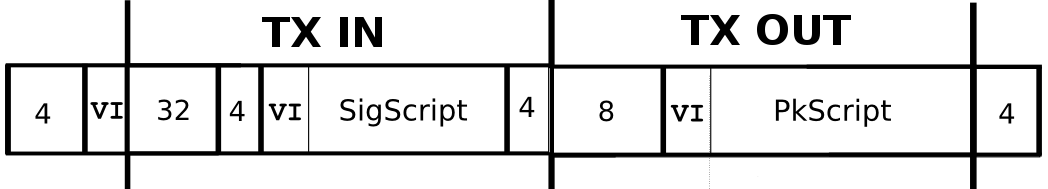
\includegraphics[width=\linewidth]{img/tx_format.png}
    \centering{
    \caption{Transaction binary format}}
\end{figure}
What every transaction does is spend a previous output by specifying an input that points to a previous output (indicated by the transaction id and number of output) and some data required to spend that output. To specify a new output to move the funds spent by the, the value of the output and the conditions to spend must be specified. This mentioned data to spend and conditions to spend is specified using a scripting language exclusive for Bitcoin technology\cite{bitcoin-wiki-script:online}. But if all transactions have to spend a previous output, when are the first outputs generated? There's a special transaction with no inputs that is the one that generates currency, but it just valid once in a block, to spend the reward (that must mutch exactly the reward value) a node receives when creating a new block, otherwise the rest of nodes in the network won't accept it as valid.


\subsection{Bitcoin scripting language}
One of the powers of Bitcoin is its stack-based scripting language, as allows to specify how funds can be spent by creating a small script in the Bitcoin scripting language\cite{bitcoin-wiki-script:online} described in the Bitcoin protocol. Therefore for a transaction to be valid, the input must refer a valid and non-spent output (also called UTXO: Unspent Transaction Output) and the input script (also called \textit{scriptSig} followed by the refered output script (also called\textit{scriptPubKey} must end succesfully with a non-empty stack. Also, the sum of outputs' values must be less than the sum of inputs' values\footnote{The difference between the sum of inputs and outputs if is greater than 0 is called the transaction \textbf{fee}, and will be rewarded along with the block reward to the node that includes the transaction in a block (in Bitcoin argot, \textit{mines} the block)}. This scripting language basically reads 1-byte opcodes that able to store (push into the stack) data, perform arithmetical operations over that, and some cryptographic operations like ECDSA signatures and hash functions. \\\\
The most used script is called P2PKH (pay-to-public-key-hash), that sets as the conditions for spending an output (the \textit{scriptPubKey}) to specify a public key whose hash matches the specified one and a signature with that public key of the transaction spending the output. The input script (the \textit{scriptSig}) therefore must contain a valid public key whose hash matches the specified in the output script and a valid signature performed with the private key paired to that public key. The hash of a public key needed in the mentioned output script to specify the spend conditions, prefixed by a version byte (that determines the network it is valid and that the type of data is a hash of a public key) suffixed with a SHA-256 4-byte checksum of that hash, all encoded in base58 is a Bitcoin address, commonly used to pay units of currency to another user who reveals their address to be paid.\\\\
But as said before, the Bitcoin scripting language allows us to code any script to specify the spend conditions and any script to specify the data to spend following those conditions. Here is when P2SH (pay-to-script-hash) comes. This method of payment allows us to create an smart contract by defining an script where we specify the conditions to spend the output (called the \textit{redeemScript}) and create an output paying to this script hash. Therefore to spend that output, we must reveal the \textit{reedemScript} and often specify also data that the script needs to be spent, like some signatures (multisig P2SH) or a hash preimage, or whatever we design\footnote{Despite we could technically specify any output and input script so that if the input script followed by the output script return a valid result (succesfully executed with non-empty stack or False at the top of the stack), if we don't use either P2PKH or P2SH, our transaction would be non-standard and probably not accepted by the network nodes}.
\section{Unidirectional Payment Channels}
The first step, once understood how Bitcoin transactions work and how we can develop smart contracts with them, is to design unidirectional payment channels. This channels, also called simple micropayment channels were first defined by Mike Hearn and Jeremy Spilman\cite{bitcoin-wiki-contract:online} and basically define two users, one who pays (payer) incrementally some amounts to the other (payee).
\subsection{The scheme}
Every channel has three phases: \textbf{funding}, where the founder or channel payer put some units of currency they own into a smart contract (we use a P2SH to pay to a \textit{redeemScript}), \textbf{payments} where the payer creates transactions that incrementally pay more to payee spending the funding output (so the payee just keeps the one that pays more to them, as just one of all the payment transactions is valid) and the \textbf{closure} where the channel is closed either because its expiry date is coming (and the payee signs and broadcasts the latest received transaction) or because a user acted maliciously. Therefore the scheme is to create a funding transaction paying to a smart contract that allows spending it using a multisig (so the payer creates transaction to pay to the payer that signs prior sending it to them) or after a certain time by the founder (as if the payee doesn't collaborate and doesn't perform the multisig funds could be locked forever). This can be achieved either by creating a smart funding transaction that includes the expiry condition or a multisig funding transaction and a refund transaction that is signed by both and allows to be spent after a certain time. We opted for a single smart transaction in order to simplify the process. Summarizing, the most important part is the funding smart contract, as must allow a refund after a certain time in case the payee does not collaborate so the payer can recover the funds and also to pay incremental amounts to the payee.
\subsection{The smart contract}
In order to create a transaction that spends some funds of the payer and the output pays to a smart contract that requires a multisig for being spent (and will be used to perform payments) or just a signature after certain time (to prevent from funds being locked if payee doesn't collaborate), our proposal\footnote{Along with Carlos Gonzalez Cebrecos} was to create a transaction funding this \textit{redeemScript}:
\begin{center}
\code{OP\_IF <time> OP\_CHECKLOCKTIMEVERIFY OP\_DROP <PubKeyPayer1> OP\_CHECKSIG OP\_ELSE OP\_2 <PubKeyPayer2> <PubKeyPayee> OP\_2 OP\_CHECKMULTISIG OP\_ENDIF}
\end{center}
Note that the payer both owns private key of \code{<PubKeyPayer(1/2)>} and the payee holds the private key of \code{<PubKeyPayee>}. 
\subsection{Channel operations}
With this smart contract script, we could create and test after that all the transactions for the channel:
\begin{itemize}
    \item \textbf{Funding}: A transaction spending a payer's P2PKH \textit{scriptSig} and with a P2SH output paying to the previously mentioned redeem script hash
    \item \textbf{Payment}: A transaction signed by both parties (firstly signed by the payer and then sent to the payee missing its signature to be valid) spending the redeem script with the \code{OP\_CHECKMULTISIG} statement specifying an \code{OP\_FALSE} and whose outputs are P2PKH \textit{scriptPubKeys} to the payed and to the payee as a return. Each payment transaction must pay more than the previous one to the payer, as the payer will always hold the one that pays more to them. In case of wanting the payer to receive less than the previous transaction, we need a bidirectional payment channel.
    \item \textbf{Refund}: A transaction signed by the payer, and with \code{nLocktime}\footnote{We require the use of the \code{nLocktime} transaction field in order to make the script \code{OP\_CHECKLOCKTIMEVERIFY} work as specified in BIP-65\cite{bip-65:online}} field set after the \code{<time>} field specified in the script, spending the transaction with just its signature as specifies to pay with the first block of the redeem script with an \code{OP\_TRUE} and whose output is a P2PKH output to an address the founder owns.
    \item \textbf{Closure}: The same transaction as the payment can act as a closure if broadcasted to the network previously signed by the payee. It has to be sent by the payed user before the expiry time or the payer could use the refund transaction so all payment transactions would be invalid as those funds would be already spent by the refund transaction.
\end{itemize}
\subsection{The protocol}
All this transactions must be created following a secure protocol that ensures all users are secure creating and operating the channel without any of them trusting the other. The protocol to establish a unidirectional payment channel between Alice (the payer) and Bob (the payee) would be the following:
\begin{figure}[h]
    \begin{center}
        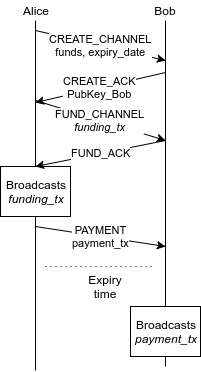
\includegraphics[height=7.5cm]{unidir-pc}
        \caption{Unidirectional payment channel protocol}
    \end{center}
\end{figure}
Alice requests opening a channel and specifies the funds of the channel (maximum amount Alice can pay to Bob) and the expiry date of it. If Bob agrees on the channel creation, he sends its public key so that Alice can create the funding transaction. Once the funding transaction is created, Alice sends the transaction to Bob along with the redeem script, so he can trace it and verify the contract is correct. Bob sends an acknowledge to Alice if wants to proceed with the channel opening (a signed one with Bob's key so Alice can verify the acknowledge is real). Alice eventually can broadcast the funding transaction to the Bitcoin network. Once the transaction is confirmed, Alice can create payment transactions, sign them and send them to Bob privately. When the expiry date is getting over, Bob will close the channel by broadcasting the latest received payment transaction to the Bitcoin network (after signing it with its key).

\section{Bidirectional payment channels}
The problem with above channels is that just the payer can pay incrementally amounts of currency unit to the payee. What if we want the channel to be duplex so that both parties can send amounts of currency in both ways? In this work we researched following the solution proposed by Christian Decker and Roger Wattenhofer\cite{decker2015fast} that is to basically to create a duplex payment channel by using two unidirectional payment channels linked together, one in each direction. Another popular solution proposed is the Lightning Network, that uses a more complex structure to build a duplex payment channel\cite{poon2015bitcoin}
\subsection{The scheme}
As said previously, the idea is to use two unidirectional payment channels, one in each direction, so that we can pay in both directions. To do that, in the funding transaction, there must be two inputs and two outputs. One input and one output per user. The Alice input spent value minus fees will be the first output value, where the output will pay to the same redeem script as the unidirectional channel. This will be the channel used by Alice to pay to Bob. The second input and output will be constructed using the same scheme for Bob to pay Alice. The rest of the payment channel would work the same way that in a unidirectional channel, where each transaction spends an output or another depending if Alice is paying to Bob or viceversa.
\subsection{The protocol}
In order to create the duplex payment channel, the following protocol must be followed in order for the channel to be secure:
\begin{figure}[h]
    \begin{center}
        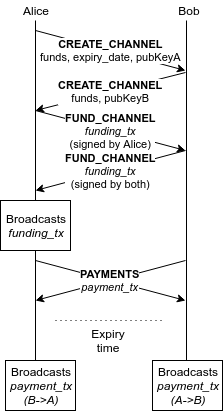
\includegraphics[height=10.5cm]{bidir-pc}
        \caption{Bidirectional payment channel protocol}
    \end{center}
\end{figure}
We can see the protocol is similar to the unidirectional payment channel. In this example, Alice starts the request for the creation of the payment channel, but Bob could also send the request, inverting the communications until the payments section. The basic protocol consists in Alice sending the request to Bob for the channel creation, as happened with the unidirectional channel with the funds Alice desires to pay Bob, but also including his public key so that Bob can verify the funding transaction created. If Bob agrees with the channel creation, replies with his public key to create the output for Alice paying to Bob and the funds that Bob wants to use to fund his channel to pay Alice. Once Alice has all data, can create the funding transaction with the two outputs and his input, and sign her input (indicating \code{SIGHASH\_ALL} meaning that signs the transaction containing the two outputs). Alice sends the partially completed transaction (along with the redeem scripts) to Bob. Bob checks the transaction is correct and adds his input signed, returning the fully signed transaction to Alice as a final acknowledge for creating the channel. Once Alice receives the transaction, checks that is valid and broadcasts the transaction to the network. Now payments spending the Alice output to pay to Bob and the Bob output to pay to Alice can be performed creating offchain transactions. To close the channel, both Bob and Alice have to release the latest received payment transactions before the channel expiry to close the channel.
\subsection{Channel operations}
The same operations applied for the unidirectional payment channel would be valid (despite the transaction for funding being slightly different with an added input and output for the second way channel).
\subsection{Channel reset}
One thing that can happen is that either Alice or Bob spends all the funds they owned paying to the other user. In that case, the channel needs to be reset, so that the received funds from the other party can be used to continue paying to them. To do this, a solution is also described by C. Decker and R. Wattenhofer\cite{decker2015fast} and is called the invalidation tree using what it's called atomic multiparty opt-in transactions.
\subsubsection{\ \ \ \ \ Atomic multiparty opt-in}
This kind of meta-transactions are a model for creating transactions to fund smart contracts (one or more outputs) that instead of being funded by one or more inputs with a P2PKH \textit{scriptSig} owned by a user, they claim a multisig \textit{P2SH} output that has not been signed yet. This allows to first design the smart contract and once all parties agree, they sign a transaction spending one or more P2PKH to fund the multisig output claimed by the opt-in transaction and now both transactions have funded the smart contract in a secure way no matter the order of signatures.\\\\
In the case of channel resetting, this transactions are not necessary for a simple duplex payment channel, but can be used if we wish the channel to be reseted, as creating another smart contract with different conditions (like specifying different amounts) spending the opt-in transaction but with a lower locktime than the previous smart contract transaction would make the new transaction the current as the old one would have a larger locktime and therefore the current one can be spent before. This just works when specifying transactions with a lower locktime to replace the previous ones, so that renewing the expiry time couldn't be done with this kind of transactions. We can also chain opt-in transactions forming what is called an invalidation tree, where the invalidation is performed by specifying lower timelocks on each new transactions to invalidate previous ones.
\\\code{(-- OPTIONAL PROJECT FEATURE --)}
\subsection{Multihop payment channels}
Using HTLC (Hash & time locked smart contracts) we can create channels that are able to route payments from A to C by using two existent channels, from A to B and B to C.
\\\code{(-- OPTIONAL PROJECT FEATURE --)}
\section{The implementation}
In order to implement the bidirectional payment channel, a research was performed to check what Python libraries where available to develop smart contracts and therefore transactions with smart contracts. What we found is that no object-oriented and well documented library was available to create non-typical transactions (P2SH with a custom \code{redeemScript}). Because of that, we implemented a new library / framework to create easily customized transactions using the Bitcoin protocol information and it's implementation details\cite{bitcoin-org-developer:online, bitcoin-wiki-proto:online}.
\subsection{Our Bitcoin framework}
To implement our framework, we decided to create a series of modules and classes oriented towards to the puzzle-friendlyness property: all objects / classes must be able to be serialized / deserialize into / from an array of bytes compatible with the Bitcoin protocol. We just implemented to save time, but, the strictly necessary modules and classes needed for this project development, but setting the base for developing a well designed, usable and easy to understand Bitcoin Python library that aims new developers to create smart contracts in the Bitcoin network.
\subsection{Developing progress}
The framework started with the ability to create an empty valid transaction and after that implementing all the fields necessary, composing each field of another subfields to allow the mentioned puzzle-friendlyness. The latest developed part of the framework was part of the Bitcoin scripting language (that is in constant development) to implement the needed opcodes to create the smart contracts.\\\\
Once the framework allowed to create valid transactions (that required special focus on cryptography functions and its serialization), we tested basic P2PKH transactions created with the framework and a P2SH multisig transaction. After that, the OP\_CHECKLOCKTIME verify was implemented and tested and a unidirectional payment channel was created.\\\\
After all development and testing finished for the creation of valid and functional unidirectional payment channels, I started developing the Bidirectional Payment Channel as specified in the previous chapter of this document.
\subsection{The duplex channel implementation}
\\\code{(-- TODO --)}
% An example of a floating figure using the graphicx package.
% Note that \label must occur AFTER (or within) \caption.
% For figures, \caption should occur after the \includegraphics.
% Note that IEEEtran v1.7 and later has special internal code that
% is designed to preserve the operation of \label within \caption
% even when the captionsoff option is in effect. However, because
% of issues like this, it may be the safest practice to put all your
% \label just after \caption rather than within \caption{}.
%
% Reminder: the "draftcls" or "draftclsnofoot", not "draft", class
% option should be used if it is desired that the figures are to be
% displayed while in draft mode.
%
%\begin{figure}[!t]
%\centering
%\includegraphics[width=2.5in]{myfigure}
% where an .eps filename suffix will be assumed under latex, 
% and a .pdf suffix will be assumed for pdflatex; or what has been declared
% via \DeclareGraphicsExtensions.
%\caption{Simulation Results}
%\label{fig_sim}
%\end{figure}

% Note that IEEE typically puts floats only at the top, even when this
% results in a large percentage of a column being occupied by floats.
% However, the Computer Society has been known to put floats at the bottom.


% An example of a double column floating figure using two subfigures.
% (The subfig.sty package must be loaded for this to work.)
% The subfigure \label commands are set within each subfloat command, the
% \label for the overall figure must come after \caption.
% \hfil must be used as a separator to get equal spacing.
% The subfigure.sty package works much the same way, except \subfigure is
% used instead of \subfloat.
%
%\begin{figure*}[!t]
%\centerline{\subfloat[Case I]\includegraphics[width=2.5in]{subfigcase1}%
%\label{fig_first_case}}
%\hfil
%\subfloat[Case II]{\includegraphics[width=2.5in]{subfigcase2}%
%\label{fig_second_case}}}
%\caption{Simulation results}
%\label{fig_sim}
%\end{figure*}
%
% Note that often IEEE papers with subfigures do not employ subfigure
% captions (using the optional argument to \subfloat), but instead will
% reference/describe all of them (a), (b), etc., within the main caption.


% An example of a floating table. Note that, for IEEE style tables, the 
% \caption command should come BEFORE the table. Table text will default to
% \footnotesize as IEEE normally uses this smaller font for tables.
% The \label must come after \caption as always.
%
%\begin{table}[!t]
%% increase table row spacing, adjust to taste
%\renewcommand{\arraystretch}{1.3}
% if using array.sty, it might be a good idea to tweak the value of
% \extrarowheight as needed to properly center the text within the cells
%\caption{An Example of a Table}
%\label{table_example}
%\centering
%% Some packages, such as MDW tools, offer better commands for making tables
%% than the plain LaTeX2e tabular which is used here.
%\begin{tabular}{|c||c|}
%\hline
%One & Two\\
%\hline
%Three & Four\\
%\hline
%\end{tabular}
%\end{table}


% Note that IEEE does not put floats in the very first column - or typically
% anywhere on the first page for that matter. Also, in-text middle ("here")
% positioning is not used. Most IEEE journals use top floats exclusively.
% However, Computer Society journals sometimes do use bottom floats - bear
% this in mind when choosing appropriate optional arguments for the
% figure/table environments.
% Note that, LaTeX2e, unlike IEEE journals, places footnotes above bottom
% floats. This can be corrected via the \fnbelowfloat command of the
% stfloats package.



\section{Conclusion}
\\\code{(-- TODO (Main point: switch to Ethereum, also flippening is happening :) --)}



% if have a single appendix:
%\appendix[Proof of the Zonklar Equations]
% or
%\appendix  % for no appendix heading
% do not use \section anymore after \appendix, only \section*
% is possibly needed

% use appendices with more than one appendix
% then use \section to start each appendix
% you must declare a \section before using any
% \subsection or using \label (\appendices by itself
% starts a section numbered zero.)
%


% \appendices
% \section{Proof of the First Zonklar Equation}
% Appendix one text goes here.

% you can choose not to have a title for an appendix
% if you want by leaving the argument blank
% \section{}
% Appendix two text goes here.


% use section* for acknowledgement
\ifCLASSOPTIONcompsoc
  % The Computer Society usually uses the plural form
  \section*{Acknowledgments}
\else
  % regular IEEE prefers the singular form
  \section*{Acknowledgment}
\fi


This work couldn't have been possible without the collaboration with Carlos Gonzalez Cebrecos, another student performing a similar project that coworked developing our Bitcoin framework and solving some Bitcoin and related technologies doubts along with our tutors Jordi Herrera Joancomarti, Sergi Delgado and Cristina Perez who introduced us in the Bitcoin world.


% Can use something like this to put references on a page
% by themselves when using endfloat and the captionsoff option.
\ifCLASSOPTIONcaptionsoff
  \newpage
\fi



% trigger a \newpage just before the given reference
% number - used to balance the columns on the last page
% adjust value as needed - may need to be readjusted if
% the document is modified later
%\IEEEtriggeratref{8}
% The "triggered" command can be changed if desired:
%\IEEEtriggercmd{\enlargethispage{-5in}}

% references section

% can use a bibliography generated by BibTeX as a .bbl file
% BibTeX documentation can be easily obtained at:
% http://www.ctan.org/tex-archive/biblio/bibtex/contrib/doc/
% The IEEEtran BibTeX style support page is at:
% http://www.michaelshell.org/tex/ieeetran/bibtex/
%\bibliographystyle{IEEEtran}
% argument is your BibTeX string definitions and bibliography database(s)
%\bibliography{IEEEabrv,../bib/paper}
%
% <OR> manually copy in the resultant .bbl file
% set second argument of \begin to the number of references
% (used to reserve space for the reference number labels box)
% \begin{thebibliography}{1}
% \end{thebibliography}
\bibliography{bibliography}{}
\bibliographystyle{ieeetr}
% biography section
% 
% If you have an EPS/PDF photo (graphicx package needed) extra braces are
% needed around the contents of the optional argument to biography to prevent
% the LaTeX parser from getting confused when it sees the complicated
% \includegraphics command within an optional argument. (You could create
% your own custom macro containing the \includegraphics command to make things
% simpler here.)
%\begin{biography}[{\includegraphics[width=1in,height=1.25in,clip,keepaspectratio]{mshell}}]{Michael Shell}
% or if you just want to reserve a space for a photo:

% \begin{IEEEbiography}{Michael Shell}
% Biography text here.
% \end{IEEEbiography}

% if you will not have a photo at all:
% \begin{IEEEbiographynophoto}{John Doe}
% Biography text here.
% \end{IEEEbiographynophoto}

% insert where needed to balance the two columns on the last page with
% biographies
%\newpage

% \begin{IEEEbiographynophoto}{Jane Doe}
% Biography text here.
% \end{IEEEbiographynophoto}

% You can push biographies down or up by placing
% a \vfill before or after them. The appropriate
% use of \vfill depends on what kind of text is
% on the last page and whether or not the columns
% are being equalized.

%\vfill

% Can be used to pull up biographies so that the bottom of the last one
% is flush with the other column.
%\enlargethispage{-5in}



% that's all folks
\end{document}


